\chapter{Brechungsindex von Glas}
\label{v:9}

In diesem Versuch untersuchen Sie die wellenlängenabhängige Beugung (Dispersion) von Licht in einem Glasprisma.

%------------------------------------------------
\section{Stichworte}
%------------------------------------------------

Reflexion; Brechungsgesetz nach Snellius; Huygenssches Prinzip; Dispersion; Brechungsindex; Minimalablenkwinkel.
%
%------------------------------------------------
\section{Literatur}
%------------------------------------------------

Gehrtsen, Kapitel 9.1.2 - 9.1.5
%
%------------------------------------------------
\section{Anwendungsbeispiele}
%------------------------------------------------
%
Optische Instrumente wie Linsen, Lichtleiter und Prismen werden seit jeher aus Glas oder Glas-ähnlichen Stoffen hergestellt. Ihre Funktion als optische Instrumente beruht dabei auf der Ausnutzung der unterschiedlichen Lichtgeschwindigkeit in Medien mit unterschiedlichem Brechungsindex $n$.\\
Luft wird dabei im Praktikum vereinfachend der Brechungsindex $n_{Luft} = 1$ zugeordnet. Das diese Annahme nicht immer stimmt sehen Sie am Flimmern der Luft über einer Flamme oder heißen Oberfläche, bzw. am Phänomen der Fata Morgana. 
%
%------------------------------------------------
\section{Theoretischer Hintergrund}
%------------------------------------------------

Fällt Licht auf die Grenzfläche zwischen zwei Medien (z.B. Luft und Glas), so kann es entweder reflektiert werden oder es dringt unter Änderung von Richtung, Geschwindigkeit und Wellenlänge ein. Ein Maß für diese Änderung ist der Brechungsindex $n$. Die Tatsache, dass $n$ für verschiedenfarbiges Licht verschieden ist, bezeichnet man als Dispersion; d.h. violettes Licht (kurze Wellenlänge) wird stärker abgelenkt als rotes Licht.

\subsection{Das Huygens-Fresnel'sche Prinzip und Brechung an Grenzflächen}

Die Wellenausbreitung im homogenen Medium und auch in komplizierteren Fällen lässt sich relativ intuitiv verstehen, wenn man sich nach \textit{Huygens} vorstellt, dass in jedem Punkt einer Wellenfront ein Streuzentrum sitzt, von welchem Kugelwellen (\textit{Elementarwellen}) ausgehen. Diese überlagern sich dann zu einer neuen Wellenfront.\\

\noindent
Diese Vorstellung kann man nachvollziehen, wenn man sich klar macht, wie das einfallende Licht die Atome der Materie beeinflusst. Licht besteht aus einer sich ausbreitenden elektromagnetischen Welle. Das bedeutet, dass mit dem Lichtstrahl ein sich schnell veränderndes elektrisches Feld einhergeht. Die Frequenz der Änderung des elektrischen Feldes ist dieselbe wie die, die wir dem Licht zuschreiben. Dieses elektrische Feld übt nun eine Kraft auf die Hüllenelektronen der Atome aus, indem es diese negativ geladenen Elektronen in Richtung des positiven elektrischen Feldes zu ziehen, es entsteht ein elektrisches Dipolmoment im Atom oder Molekül. Die schnellen Wechsel des elektrischen Feldes zwingen den Dipol dazu, mit derselben Frequenz zu schwingen. er ruft dadurch ein selbst ein oszillierendes elektrisches Feld hervor, welches dem Feld des einfallenden Lichtstrahls entgegengesetzt ist und dieses deshalb auslöscht. Gleichzeitig emittiert der Dipol aufgrund seiner Schwingung selbst wieder eine elektromagnetische Welle, welche dieselbe Frequenz hat, wie der ursprüngliche Lichtstrahl. Das sind die oben erwähnten Elementarwellen. Die von vielen Dipolen an der Oberfläche ausgesandten Elementarwellen überlagern sich nun konstruktiv und bilden eine ebene Wellenfront, wenn der Abstand zur Oberfläche groß gegenüber der Wellenlänge ist. Damit senden die vielen Dipole einen neuen Lichtstrahl aus, der dieselbe Frequenz hat wie der einfallende, sich jedoch in eine andere Richtung ausbreitet.\\

\noindent
Fällt eine ebene Welle schräg auf die ebene Grenze zwischen zwei Medien, in denen die Wellen unterschiedliche Ausbreitungsgeschwindigkeiten $c_1$ und $c_2$ haben, so haben die Elementarwellen in den beiden Medien nach einer bestimmten Zeit unterschiedliche Radien, welche sich wie $c_1/c_2$ verhalten (s. Abb. \ref{fig:brechung}). Damit nehmen die Überlagerungen der Elementarwellen, welche in dem jeweiligen Medium wieder ebene Wellenfronten bilden, verschiedene Winkel zum Lot auf die Grenzfläche ein. Bezeichnet $\alpha$ den Einfallswinkel und $\beta$ den Ausfallswinkel, dann erhalten wir das allgemeingültige Brechungsgesetz nach Snellius:
\begin{equation} \label{eq:Brechungsgesetz}
\frac{\sin\alpha}{\sin\beta} = \frac{c_1}{c_2}
\end{equation}

\begin{figure}[hb]
	\centering
		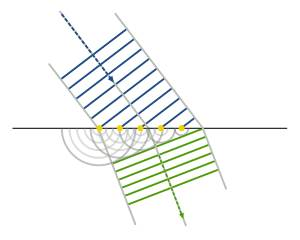
\includegraphics[width=.5\textwidth]{Abbildungen/Brechung.jpg}
	\caption{Lichtbrechung mit Huygens'schem Prinzip. Im Medium oberhalb der Grenzfläche beträgt die Lichtgeschwindigkeit $c_1$, darunter $c_2$. \\
	Quelle: Wikimedia, Autor Arne Nordmann}
	\label{fig:brechung}
\end{figure}

\subsection{Brechungsindex und Snellius'sches Brechungsgesetz}

Der Brechungsindex $n$ eines Mediums kann über die Geschwindigkeit der Lichtwellen in diesem Medium definiert werden als:
\begin{equation}
n = \frac{c_0}{c_m}\, ,
\end{equation}
wobei $c_0$ die Lichtgeschwindigkeit im Vakuum bezeichnet und $c_m$ die Lichtgeschwindigkeit im Medium.\\

\noindent
Mit dieser Definition wird aus Gleichung \ref{eq:Brechungsgesetz} das \textit{Snellius'sche Brechungsgesetz}
\begin{equation} \label{eq:Snellius}
\frac{\sin\alpha_1}{\sin\alpha_2} = \frac{n_2}{n_1} = \frac{c_1}{c_2}
\end{equation}

\subsection{Totalreflexion}

Aus dem Brechungsgesetz (Gl. \ref{eq:Snellius}) kann man sehen, dass es einen Einfallswinkel $\alpha_1$ gibt, bei dem Reflexion unmöglich wird.\\
Da beim Übergang vom optisch dichteren Medium (mit größerem Brechungsindex) ins optisch dünnere Medium das Licht vom Lot auf die Grenzfläche weg gebrochen wird ist der Ausfallswinkel $\alpha_2$ immer größer als der Einfallswinkel. Wird der Ausfallswinkel entsprechend Gl. \ref{eq:Snellius} gleich 90$^{\circ}$, so läuft das Licht entlang der Grenzfläche. Wird der Einfallswinkel noch größer erscheint die Grenzfläche reflektierend und das Licht wird gemäß dem Reflexionsgesetz 'Einfallswinkel gleich Ausfallswinkel' wieder in das optisch dichtere Medium zurück reflektiert.\\
Damit ist klar, dass für den Einfallswinkel, unter dem Totalreflexion auftritt, gelten muss:
\begin{equation}
	\sin\alpha_1 \geq \frac{n_2}{n_1}
\end{equation}

\subsection{Dispersion}

In vielen Medien, wie z. Bsp. Wasser und Glas, hängt der Brechungsindex des Mediums von der Wellenlänge, bzw. der Frequenz, des Lichtes ab: $n = n(\lambda)$. Diese Tatsache nennt man \textit{Dispersion}. Aus historischen Gründen bezeichnet man den Fall, dass der Brechungsindex mit abnehmender Wellenlänge zunimmt $\left( \frac{dn}{d\lambda}<0\right)$ als \textit{normale Dispersion}, den umgekehrten Fall $\left( \frac{dn}{d\lambda}>0\right)$ als \textit{anomale Dispersion} (Beachte: nicht anormal, sondern anomal).\\
In diesen Fällen gilt immer noch das Brechungsgesetz nach Snellius, so lange man für jede betrachtete Wellenlänge den korrespondierenden Brechungsindex einsetzt.\\

\noindent
Das klassische Beispiel für Dispersion in der Natur ist der Regenbogen. Wir sehen einen Regenbogen vor uns, wenn die Sonne nicht zu hoch und hinter uns steht und es vor uns regnet. In diesem Fall tritt ein weißer Lichtstrahl von der Sonne in einen Wassertropfen ein, wobei es zur Dispersion kommt. Das Licht wird an der uns abgewandten Seite des Tropfens total reflektiert und tritt in unsere Richtung wieder aus dem Tropfen aus, wobei die Dispersion wieder auftritt. Da kurzwelliges Licht (blau) stärker gebrochen wird als langwelliges (rot), kann man aus genügend großer Entfernung die verschiedenen Farben des Sonnenlichtes unter verschiedenen Winkeln, also scheinbar an verschiedenen Orten am Himmel sehen: Ein Regenbogen.

\subsection{Ein paar Worte zum Prisma}

Wenn ein Lichtstrahl symmetrisch durch das Prisma hindurchgeht, d.h. parallel zur Basis (s. Abb. \ref{fig:prisma2}), erfährt er die kleinste Ablenkung (Minimal-Ablenkungswinkel). In diesem Fall lässt sich eine geometrische Beziehung zwischen dem Brechungsindex $n$ des Prismas, dem brechenden Winkel $\epsilon$ des Prismas und dem Minimalablenkungswinkel $\delta$ aufstellen:
\begin{equation} \label{eq:Brechungsindex}
n = \frac{\sin\left(\frac{\delta + \epsilon}{2}\right)}{\sin\left(\frac{\epsilon}{2}\right)}
\end{equation}
Diese nennt man die \textit{Fraunhofer Formel}.\\

\noindent
Aufgrund der Dispersion des Glases hängt der Brechungswinkel von der Wellenlänge ab. Dieser Effekt wird beschrieben durch die \textit{Winkeldispersion} des Prismas:
\begin{equation}
	\frac{d\delta}{d\lambda} = \frac{\partial\delta}{\partial n} \frac{dn}{d\lambda}.
\end{equation}
Der erste Faktor kann aus der Fraunhoferschen Formel berechnet werden, der zweite $\frac{dn}{d\lambda}$ ist die Dispersion.
%------------------------------------------------
\section{Fragen zur Vorbereitung}
%------------------------------------------------

\begin{enumerate}
 %
% \item Was soll heute im Praktikum gemessen werden? Warum?
 %
 \item Welchen physikalischen Vorgang beschreibt das Snellius'sche Brechungsgesetz?
 %
 \item Wie ist der Brechungsindex definiert?
 %
 \item Wie hängen Wellenlänge und Frequenz einer Lichtwelle zusammen?
 %
 \item Was ist Dispersion?
 %
 \item Wann kann man Totalrefelxion beobachten?
 %
 \item Wie lässt sich der Winkel f"ur die Totalreflexion aus dem Snellius'schen Brechungsgesetz ableiten?
 %
 \item Wird im Prisma rotes oder blaues Licht stärker abgelenkt?
 %
\end{enumerate}

%------------------------------------------------
\section{Durchführung} 
%------------------------------------------------

\begin{minipage}{.4\textwidth}
Im Versuch wird der Brechungsindex n eines Glasprismas bestimmt, das auf einer Apparatur steht, mit der man Winkel zwischen Lichtstrahlen sehr genau messen kann.\\

\noindent
Das Fernrohr kann geschwenkt und die Stellung auf einer Gradeinteilung abgelesen werden. Die Einteilung der Scheibe ist auf 0,50\degree genau. Der Nonius umfasst 30 Skalenteile, so dass man auf eine Bogenminute genau ablesen kann.

\end{minipage}
%
\begin{minipage}{.6\textwidth}	
	\begin{center}
		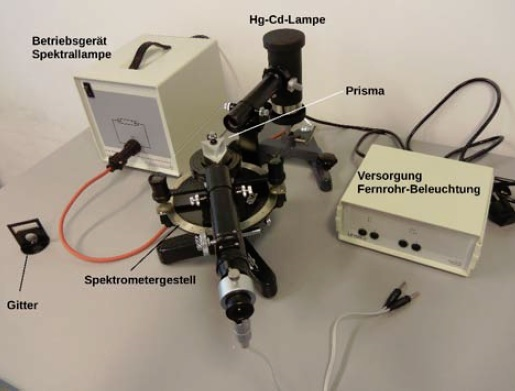
\includegraphics[width=.9\textwidth]{Abbildungen/Prismenaufbau.jpg}
	\end{center}
\end{minipage}

Der Spalt sollte aus Intensitätsgründen nicht zu eng eingestellt werden. Der Spalt sollte breiter sein als das Fadenkreuz im Fernrohr.

\begin{enumerate}
	%
	\item Verschieben Sie den Tubus des Spaltes so lange, bis Sie mit dem Fernrohr ein scharfes Bild des beleuchteten Spaltes sehen.
	%
	\item Beleuchten Sie den Spalt mit der Hg-Cd Lampe und lesen Sie auf dem Nonius den Winkel ab, unter dem Sie direkt das Bild des Spaltes sehen. \label{task:Spaltbild}
	%
	\item Stellen Sie das Prisma so in den Strahl, dass das Licht wie in Abb. \ref{fig:prisma2} gezeigt durch das Prisma fällt. Stellen Sie durch Drehen das Prisma auf den minimalen Ablenkwinkel für die gelbe Doppellinie der Hg-Cd Lampe ein. Verkleinern Sie die Spaltöffnung, bis Sie deutlich zwei Linien sehen. Notieren Sie die Winkel.
	%
	\item Arretieren Sie den Grobtrieb des Fernrohrs. 
	%
	\item Messen Sie den Ablenkwinkel der restlichen Linien im Spektrum der Hg-Cd Lampe mit dem Feintrieb des Fernrohrs. Schätzen Sie die Unsicherheit der Winkelmessung ab und notieren Sie diese. \label{task:HgSpektrum}
	%
\end{enumerate}

%------------------------------------------------
\section{Auswertung} 
%------------------------------------------------
\etodo{Musterauswertung}
\begin{enumerate}
%
 \item Korrigieren Sie die gemessenen Ablenkwinkel $\varphi$ aus Aufgabe \ref{task:HgSpektrum} um den Winkel aus Aufgabe \ref{task:Spaltbild}, um die wirklichen Ablenkwinkel $\delta$ zu bekommen.
 %
 \item Der Winkel der brechenden Kante des Prismas $\epsilon$ wird vom Hersteller mit 60\degree angegeben. Berechnen Sie aus den Ablenkwinkeln $\delta$ und dem Winkel der brechenden Kante des Prismas die jeweiligen Brechungsindizes mit Hilfe von Gleichung \ref{eq:Brechungsindex}. Berechnen Sie ebenfalls die Unsicherheit des Brechungsindex.
	%
 \item Tragen Sie die für die Hg-Cd Lampe gemessenen Brechungsindizes gegen die bekannten Wellenlängen der Spektrallinien auf.
 %
 \item Lesen Sie aus dem Diagramm die Dispersion $\frac{dn}{d\lambda}$ für blaues Licht und für gelbes Licht ab. Interpolieren Sie hierzu linear zwischen zwei geeigneten Wellenlängen. Wie groß ist die Unsicherheit?\\
	Der Hersteller gibt an:\\
	$\frac{dn}{d\lambda}|_{blau} = 2365\,\mathrm{cm^{-1}}$ sowie $\frac{dn}{d\lambda}|_{gelb} = 691\,\mathrm{cm^{-1}}$. Wie gut stimmen Ihre Werte mit den Herstellerangaben überein? Diskutieren Sie mögliche Abweichungen.
\end{enumerate}


\begin{table}[hb]
	\centering
		\begin{tabular}{lll}
			\hline
			Wellenlänge & Farbe & Intensität\\
			\hline
			643,85 nm & rot & stark\\
			579,07 nm & orangegelb & sehr stark\\
			576,96 nm & orangegelb & sehr stark\\
			546,07 nm & gelbgrün & stark\\
			508,58 nm & gelb & stark\\
			479,99 nm & blaugrün & stark\\
			467,82 nm & blau & mittel\\
			441,46 nm & blau & mittel\\
			407,78 nm & violett & stark\\
			\hline
		\end{tabular}
	\caption{Wellenlängen der Emissionslinien von Quecksilber und Cadmium}
	\label{tab:Wellenlaengen}
\end{table}

\begin{figure}[ht]
	\centering
		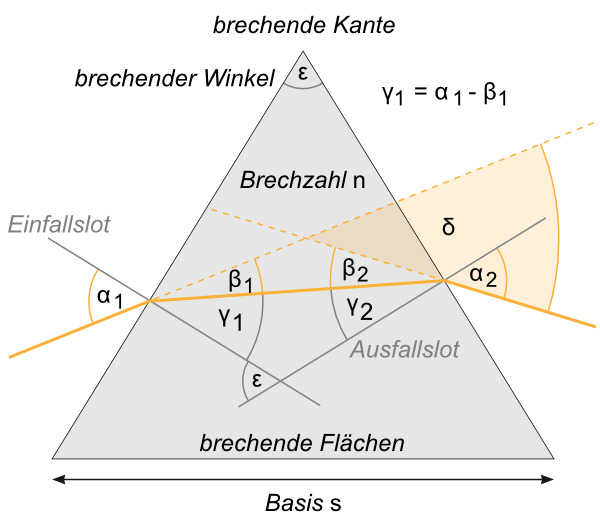
\includegraphics[width=.75\textwidth]{Abbildungen/Hauptschnitt_lpgoe.jpg}
	\caption{Hauptschnitt durch ein Prisma. Quelle: Lehrportal Universität Göttingen}
	\label{fig:prisma2}
\end{figure}